\chapter{Interaktion}
Um aus der Visualisierung ausgewählter Strukturen und Informationen eine interaktive Projektion zu erzeugen ist es erforderlich Benutzereingaben zu erfassen und auszuwerten. Dadurch wird die Modifikation der Projektion und darüber hinaus auch der Modelldaten ermöglicht.

\section{Detektion der Benutzerinteraktion}
Für die Erkennung der Benutzereingaben wird ebenfalls der Microsoft Kinect Sensor verwendet. Die Tiefeninformationen werden dabei in Form der erzeugten Punktwolken ausgewertet. Während der Benutzer das \kps in der einen Hand hält, kann die andere Hand verwendet werden um mit der Projektion zu interagieren. 
Darüber hinaus können auch weitere Personen mit dem System interagieren sofern sie bei der Benutzereingabe die Rahmenbedingungen der Funktionsweise beachten.\\
\red[Dazu wurde das in \abb{fig.zeiger} gezeigte Eingabeinstrument erstellt. Obwohl die entwickelte Erkennung der Benutzereingaben unabhängig davon funktionsfähig ist, kann die Robustheit der Anwendung dadurch deutlich verbessert werden. Integration eines Klickmechanismus ebenfalls möglich]

Der implementierte Interaktionsansatz basiert auf der Analogie zu einem Laserpointer. Ziel ist es, dem Benutzer durch Zeigebewegungen die Interaktion mit der projizierten Modellumgebung zu ermöglichen.\\
Innerhalb des Softwaremoduls \mInteraction erfolgt dafür zunächst eine Filterung der Punktwolke, da zu weit entfernte Punkte bei der Bedienung im Rahmen des handgeführten Systems nicht aus der Benutzereingabe stammen können. Alle Punkte außerhalb dieses Bereiches können für die weiteren Betrachtungen somit verworfen werden. Es entsteht der in \abb{fig.intfov} beispielhaft dargestellte zur Verfügung stehende Interaktionsbereich.\\

\begin{figure}[!ht]
	\begin{center}
		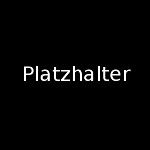
\includegraphics[scale=1.0]{spacer}
		\caption{Möglicher Interaktionsbereich}
		\label{fig.intfov}
	\end{center}
	%\vspace*{-8mm}
\end{figure}

Auf die verbleibenden Punkte wird anschließend eine Ebenendetektion nach \cite{Fischler1981} angewendet. Alle Punkte innerhalb eines definierten Abstandes werden anschließend auf die gefundene Ebene projiziert, wodurch das Messwertrauschen geglättet wird. Außerhalb liegende Punkte werden für die weiteren Schritte entfernt. Dazu gehören deutliche Ausreißer in der Interaktionsstruktur sowie weitere Artefakte in der Punktwolke.\\
Als nächstes wird eine Hüllkurve um die verbleibenden Punkte gelegt, so dass die vorhandene Struktur mittels einer äquidistanten Verteilung von Punkten angenähert werden kann. Aus dieser Hüllkurve wird der geometrische Schwerpunkt sowie der vo \kps am weitesten entfernte Punkt bestimmt. Aus diesen beiden Punkten kann nun ein Vektor berechnet werden, welcher die Zeigerichtung des Anwenders abbildet.\\
\red[\abb{fig.intdir}]

\begin{figure}[!ht]
	\begin{center}
		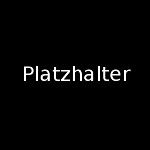
\includegraphics[scale=1.0]{spacer}
		\caption{Filterung der Punktwolke zur Bestimmung der Zeigerichtung - Subfigures: Punktewolke gesamt mit erkannter Ebene ; Projektion der Punkte auf Ebene und Entfernung von Artefakten ; Hüllkurve mit Centroid und Tip ; Erkannte Linie}
		\label{fig.intdir}
	\end{center}
	%\vspace*{-8mm}
\end{figure}

Um kleine Bewegungen des Anwenders \red[Tremor?] zu filtern wird der gleitende Mittelwert der Punkte bestimmt. Außerdem wird die Differenz zwischen zwei Punkten aus aufeinander folgenden Messungen überwacht, um zu große Sprünge in der Bewegung aufgrund von Fehldetektionen erkennen zu können.\\
Aufgrund des Implementierten Ansatzes wurde für die Kommunikation eine Nachrichtenstruktur definiert, welche die erkannte Linie abbildet. Das \mInteraction stellt die ermittelte Linie über diese Nachricht zur Verfügung und das \red[\mVisualization ?] empfängt diese.\\

Da die Kamera des Kinect Sensors auch von dem \mFovis verwendet wird besteht die Gefahr der Beeinflussung zwischen der Benutzereingabe und der lokalen Lokalisation. Um diese zu vermeiden sendet das \mInteraction Modul einen Befehl zum Pausieren der visuellen Odometrie sobald Punkte innerhalb des Interaktionsbereiches erkannt werden. Die visuelle Odometrie wird somit für die Dauer der Benutzerinteraktion unterbrochen. Sobald keine Punkte mehr innerhalb des Interaktionsbereiches detektiert werden, sendet das \mInteraction ein Signal zur Wiederaufnahme der visuellen Odometrie an das \mFovis .
Im Falle kleiner Posenänderungen während der Benutzereingabe ist die Lokalisation in der Lage die Veränderungen zu erkennen und die Pose im Anschluss an die Benutzerinteraktion zu aktualisieren.

\section{Erkennung von Befehlen}
Die Auswertung der auf Basis der Zeigebewegung ermittelten Linie erfolgt innerhalb des \red[\mVisualization]. Die detektierte Linie wird dafür zunächst aus dem Koordinatensystem der Kamera $\ks{K}$ in das globale Koordinatensystem $\ks{0}$ transformiert:

\begin{equation}
Transfomration.der.linie.in.globale.koordinaten
\end{equation}

Um zu determinieren auf welches Modellobjekt der Benutzer gezeigt hat werden entlang der Linie alle Schnittpunkte mit der Modellumgebung bestimmt. Dazu wird die Visualisierungsumgebung VTK verwendet, welche die Ermittlung von Schnittpunkten zwischen den Modell- und Linien als Funktion zur Verfügung stellt. Aus den Schnittpunkten kann somit ermittelt werden, auf welches Objekt der Benutzer gezeigt hat. Die Auswahl eines Objektes, analog eines \glqq Klick\grqq -bewegung, erfolgt durch Überprüfung der Verweildauer des simulierten Zeigers auf dem Objekt. Überschreitet diese einen definierten Grenzwert wird dies als Auswahlbefehl gewertet und das Objekt in den Zustand \textit{aktiv} versetzt. Durch Veränderung der Textur erhält der Anwender das visuelle Feedback, dass ein Objekt ausgewählt und in den neuen Status versetzt wurde (\abb{fig.intintersect}).\\

\begin{figure}[!ht]
	\begin{center}
		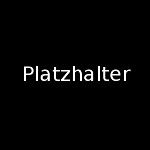
\includegraphics[scale=1.0]{spacer}
		\caption{Subfigures: Line intersection mit Modell und Abbildung des Laserpunktes - Aktivierung des Objektes}
		\label{fig.intintersect}
	\end{center}
	%\vspace*{-8mm}
\end{figure} 

Innerhalb der Modellumgebung können nun temporäre Interaktionsobjekte (\abb{fig.intarrows} \red[(a)]) eingeblendet werden, welche anschließend vom Benutzer über das gleiche Funktionsprinzip ausgewählt werden können. Alle weiteren Modellobjekte werden während dieser Phase in den Status \textit{inaktiv} versetzt. Es ist somit immer nur ein Objekt der Modellumgebung \textit{aktiv}, wodurch für den Anwender eine klare Zuordnung der Interaktionsobjekte möglich ist.

\begin{figure}[!ht]
	\begin{center}
		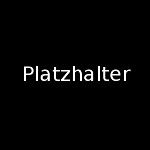
\includegraphics[scale=1.0]{spacer}
		\caption{Subfigures: Einblendung der Interaktionsobjekte und Auswahl durch Benutzer - Verschobenes Modell}
		\label{fig.intarrows}
	\end{center}
	%\vspace*{-8mm}
\end{figure} 

Durch Auswahl der Interaktionsobjekte ist der Benutzer in der Lage das aktuell als \textit{aktiv} gewählte Objekt innerhalb der Modellumgebung zu modifizieren. \abb{fig.intarrows} \red[(b)] zeigt dies am Beispiel der Translation des Modellobjektes. \red[Prinzipiell alle sechs räumlichen Freiheitsgrade möglich.]\\

Durch die Erkennung der Benutzereingabe ist der Anwender somit in der Lage Objekte der Modellumgebung auszuwählen und diese bezüglich ihrer Pose zu modifizieren. Die Integration der Interaktion in die Visualisierung ermöglicht die direkte Modifikation der zugrunde liegenden Modelldaten. Das aktualisierte Modell kann abschließend gesichert werden wodurch eine Rückführung in den virtuellen Modellierungs- und Planungsprozess ermöglicht wird.


\red[Intersection sollte auch mit Modellumgebung möglich sein!? Vielleicht Modell (obj) der Karte mit schwarzer Textur?]